%!TEX program=xelatex
\documentclass[a4paper]{article}
\usepackage{ctex}
\usepackage{geometry}
\usepackage{graphicx}
\usepackage{float}

\geometry{left=3.0cm,right=3.0cm,top=3.5cm,bottom=3.5cm}

\title{示波器实验}
\author{2017011341, 陈旭}
\date{2019 年 3 月}

\begin{document}

\maketitle

\section{实验目的}

	\par 用示波器的内置信号发生器生成以下三种波形:

	\begin{itemize}
		\item 正弦波:100 kHz,占空比为 50\%,直流电平为零,峰峰值为 4V;
		\item TTL 方波:1 MHz,占空比 50\%;
		\item 三角波:100 Hz,0-5 V,占空比 50\%。
	\end{itemize}

	\par 保存波形图并测量其频率和高低电平值。

\section{实验装置}

	\begin{itemize}
		\item 数字存储示波器(DSOX 2012A)
	\end{itemize}

\section{实验步骤}

	\subsection{生成波形}

		\par 使用示波器的“Wave Gen”功能,根据提示进行参数调节,来生成所需的波形。

	\subsection{选择信号衰减}

		\par 设置探头的衰减常数,测量超过 40 V 的信号需要使用 “$\times$10” 的探头,所以我们要生成的三种波形所对应的衰减常数应为:

		\begin{itemize}
			\item 正弦波:$\times$1
			\item TTL 方波:$\times$10
			\item 三角波:$\times$1
		\end{itemize}

		\par 同时将示波器的探头参数进行相应调整。

	\subsection{探头校准}

		\par 正确连接探头;
		\par 按下 “Auto Scale” 自动设置示波器;
		\par 进行 “无源探头检查”。

	\subsection{测量波形与参数}

		\par 按下示波器的 “Cursors”;
		\par 使用光标位移旋钮调整光标位置;
		\par 测量参数。

	\subsection{保存波形图}

		\par 使用 “Save/Recall” 功能,保存波形图及波形参数。

\section{实验结果}

	\subsection{正弦波}

	\begin{figure}[H]
		\centering
		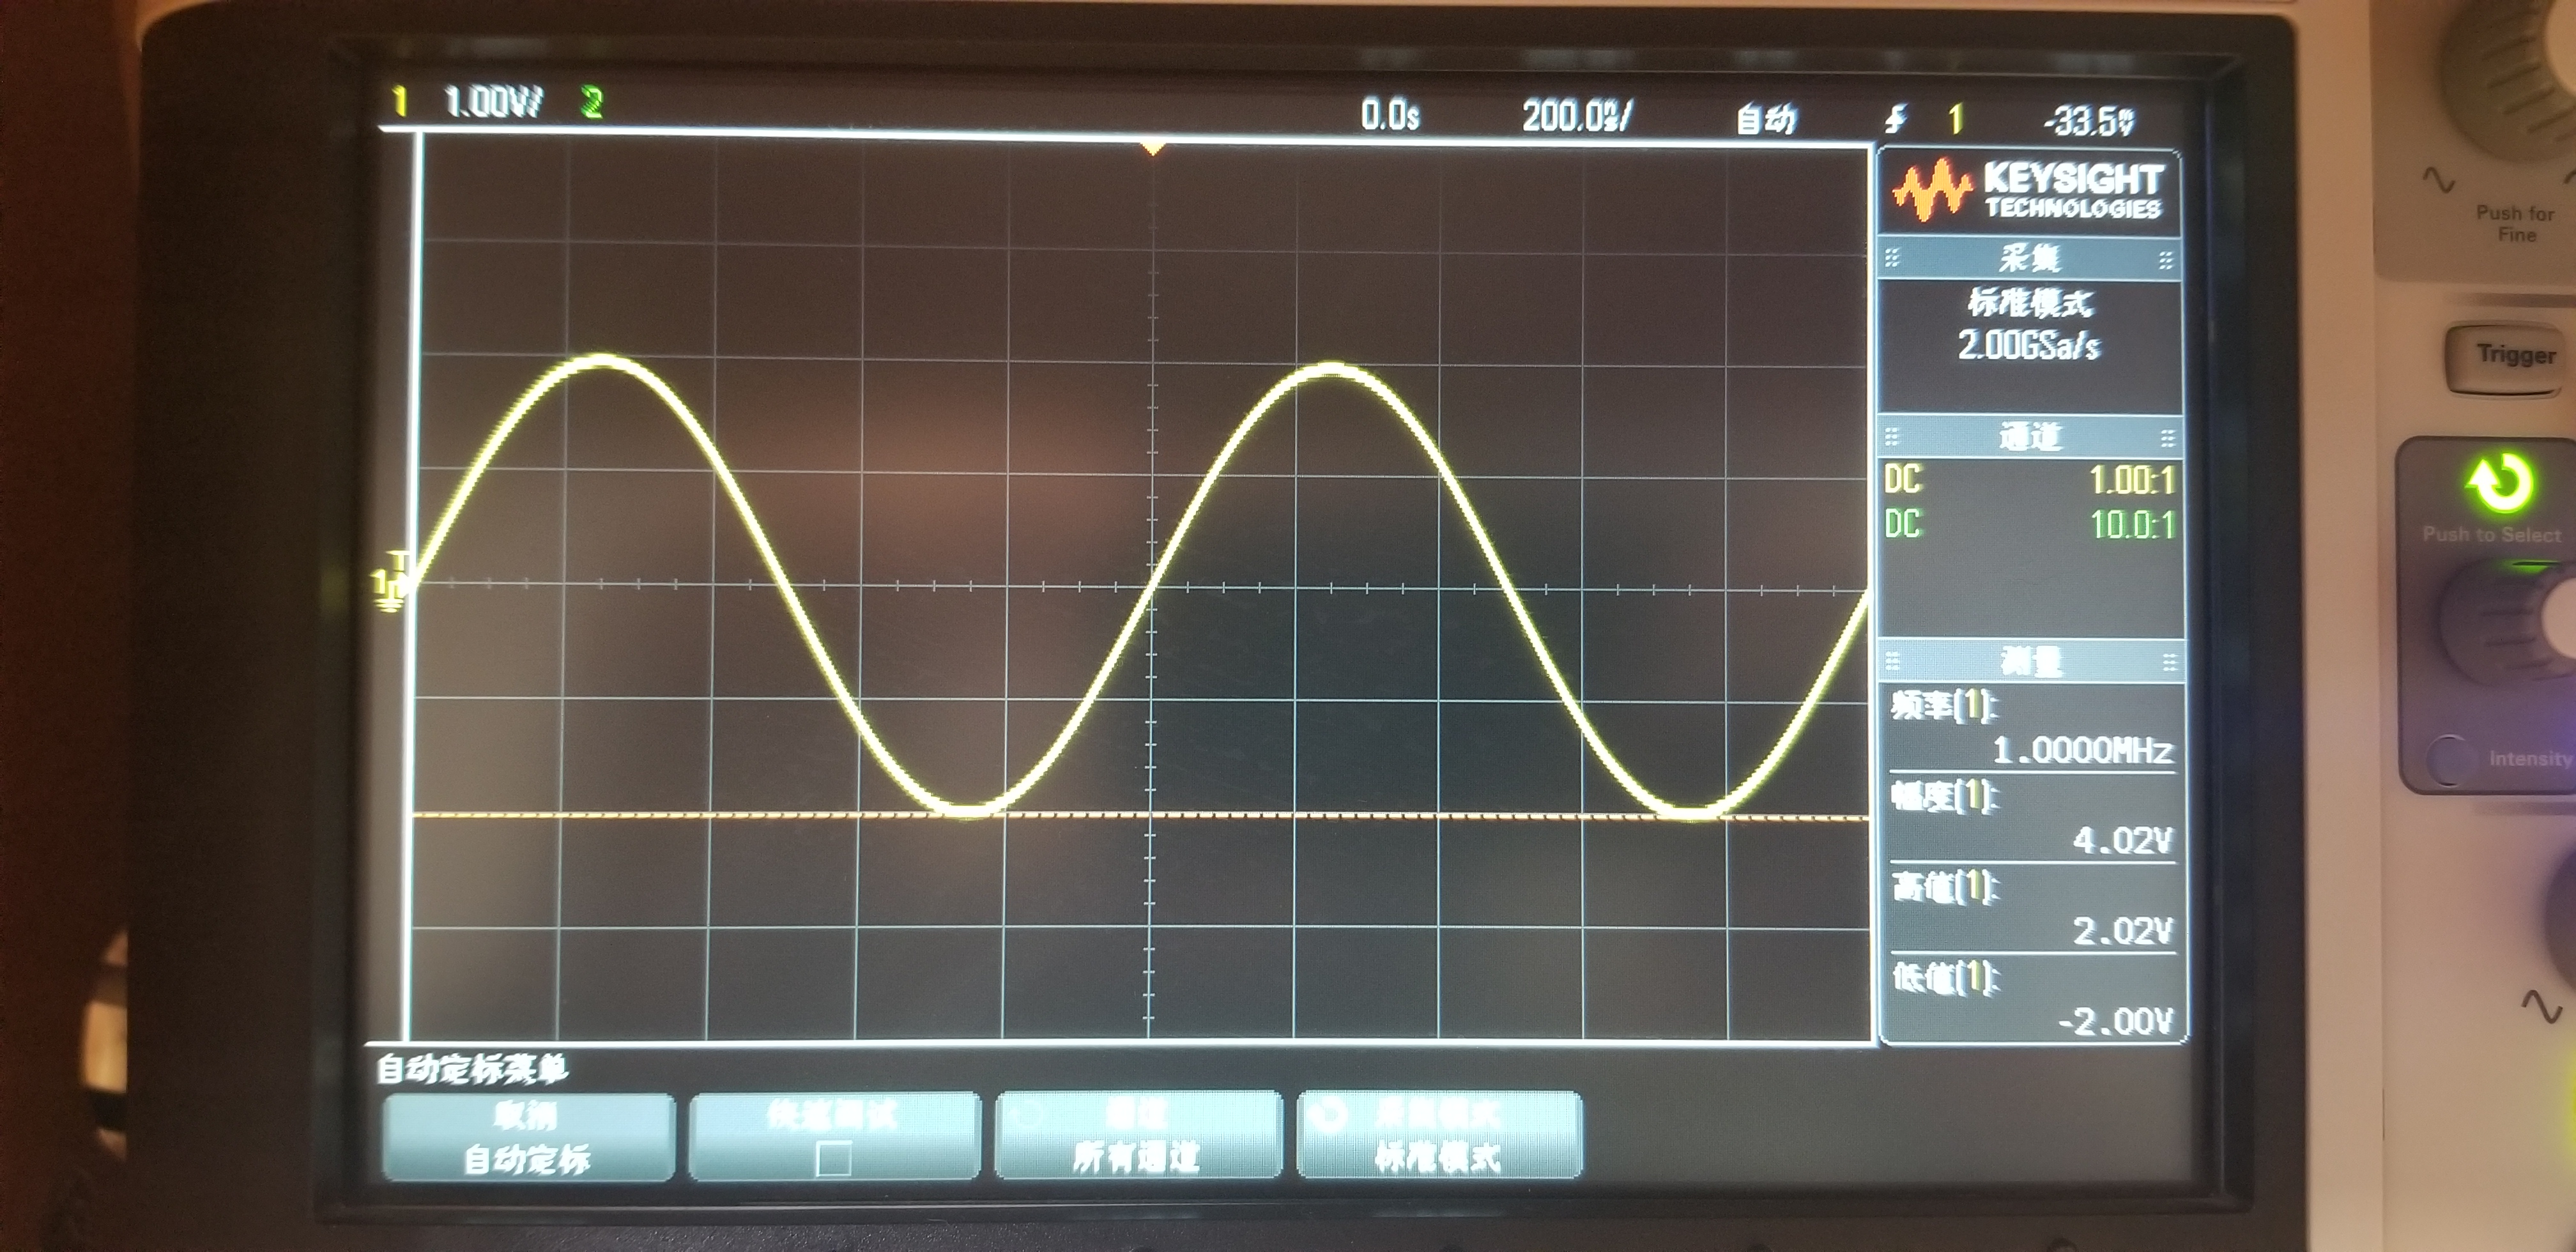
\includegraphics[width=0.7\linewidth]{figures/f1}
		\caption{正弦波}
	\end{figure}

	\subsection{TTL 方波}

	\begin{figure}[H]
		\centering
		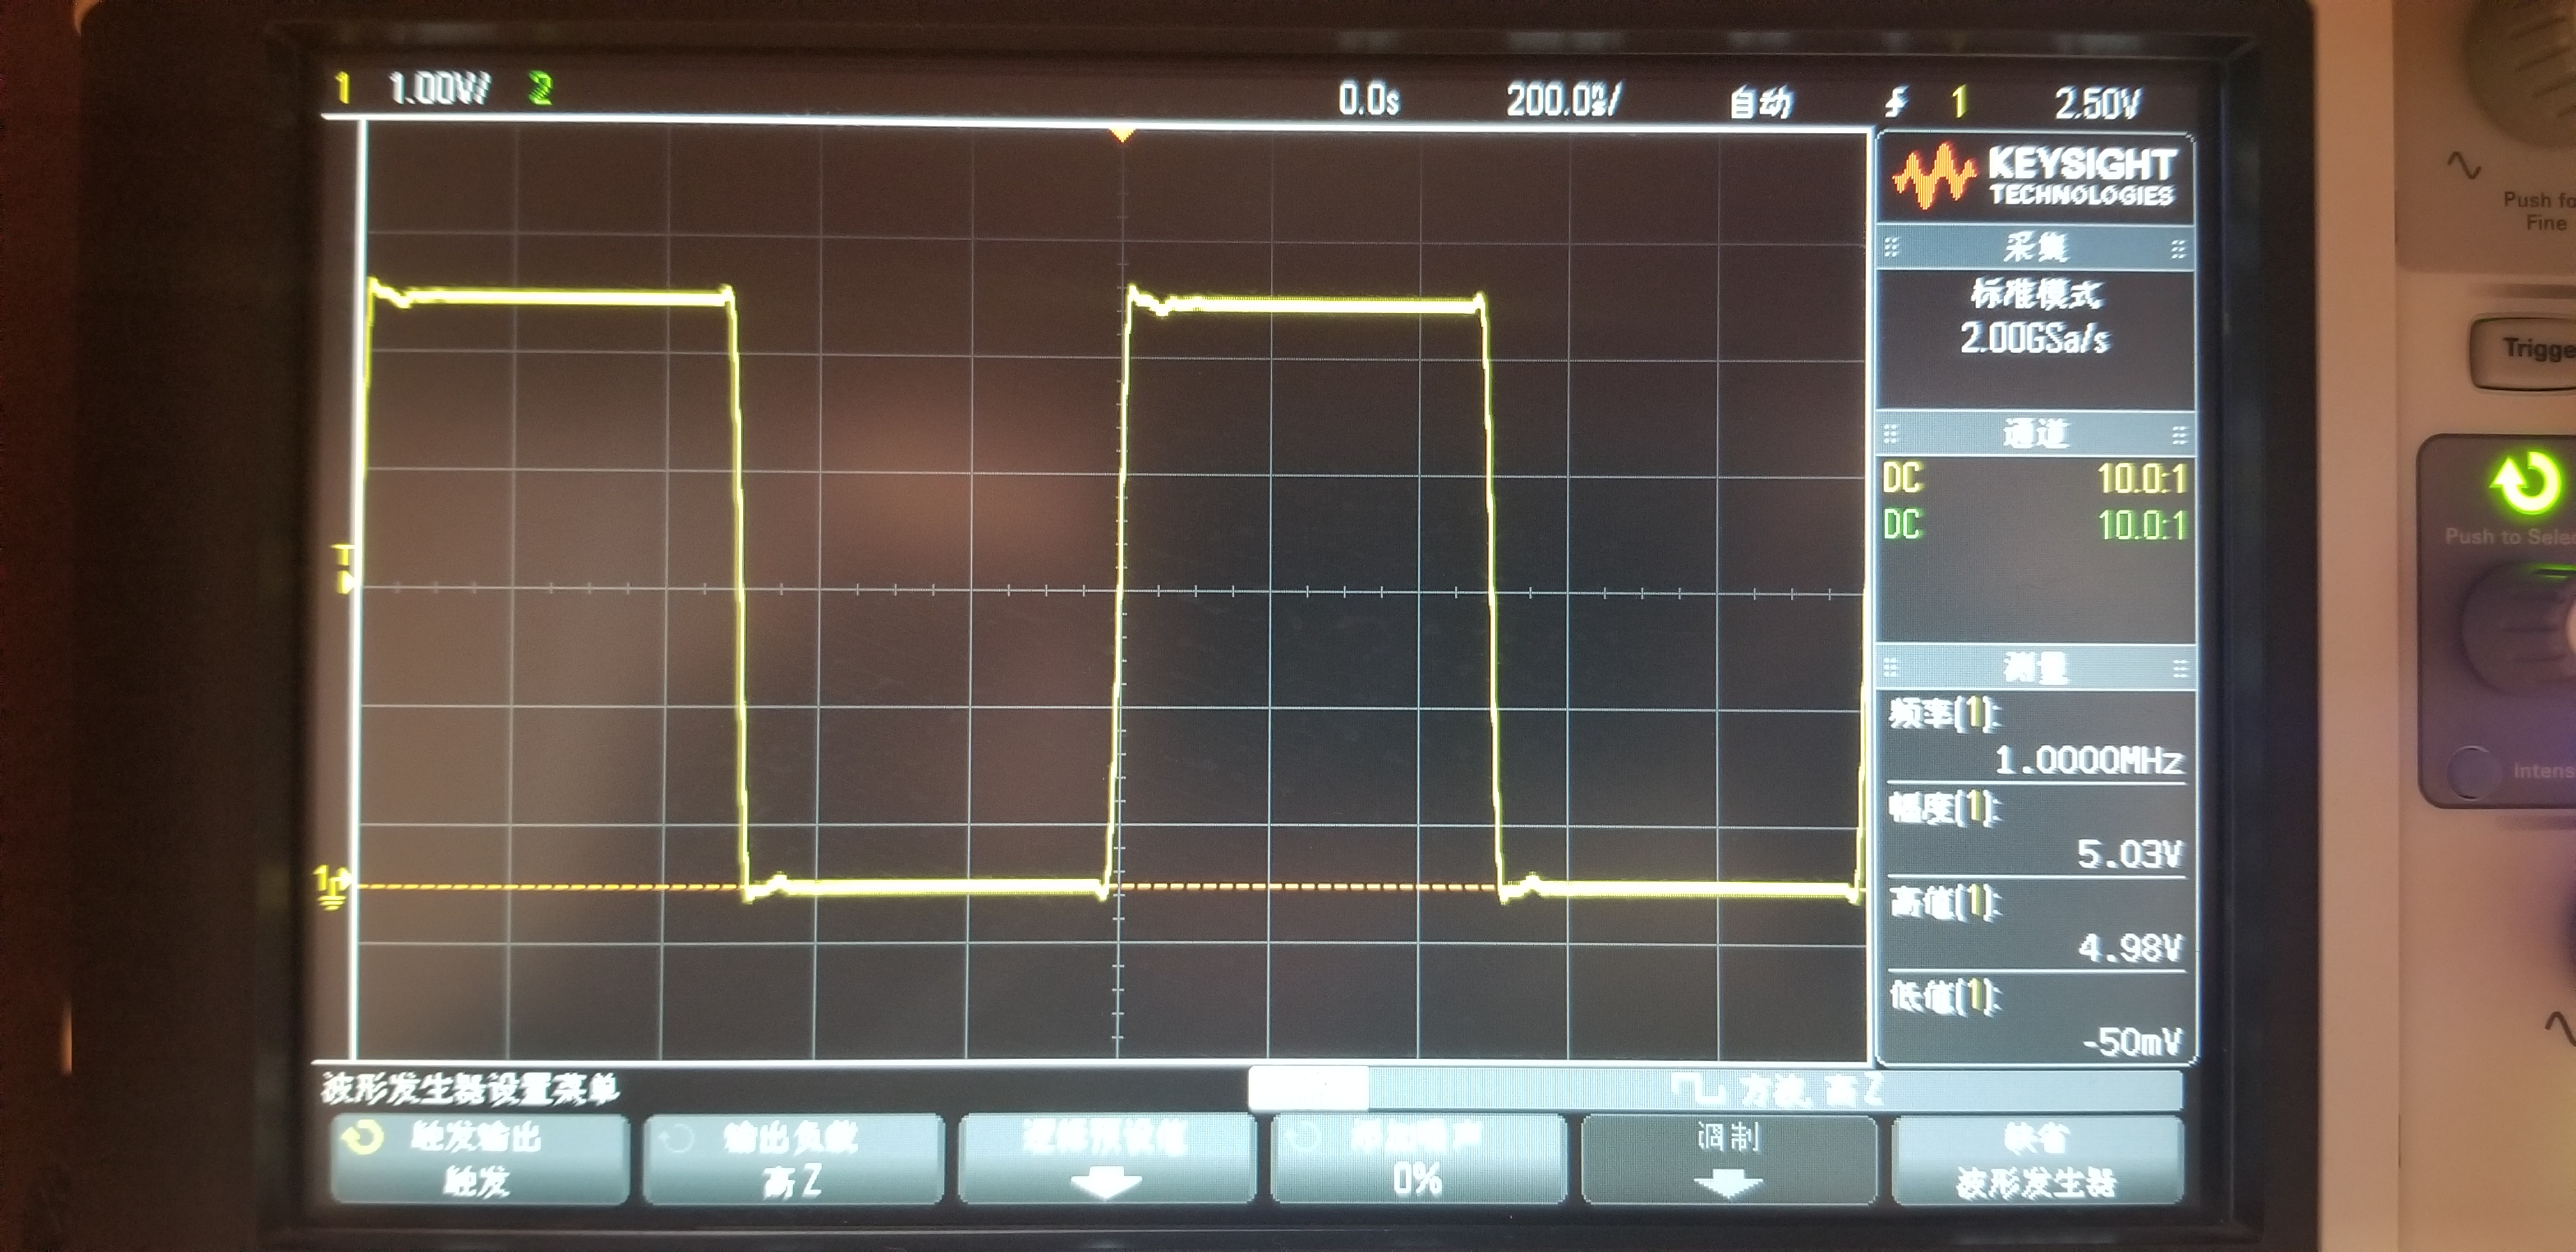
\includegraphics[width=0.7\linewidth]{figures/f2}
		\caption{TTL 方波}
	\end{figure}

	\subsection{三角波}

	\begin{figure}[H]
		\centering
		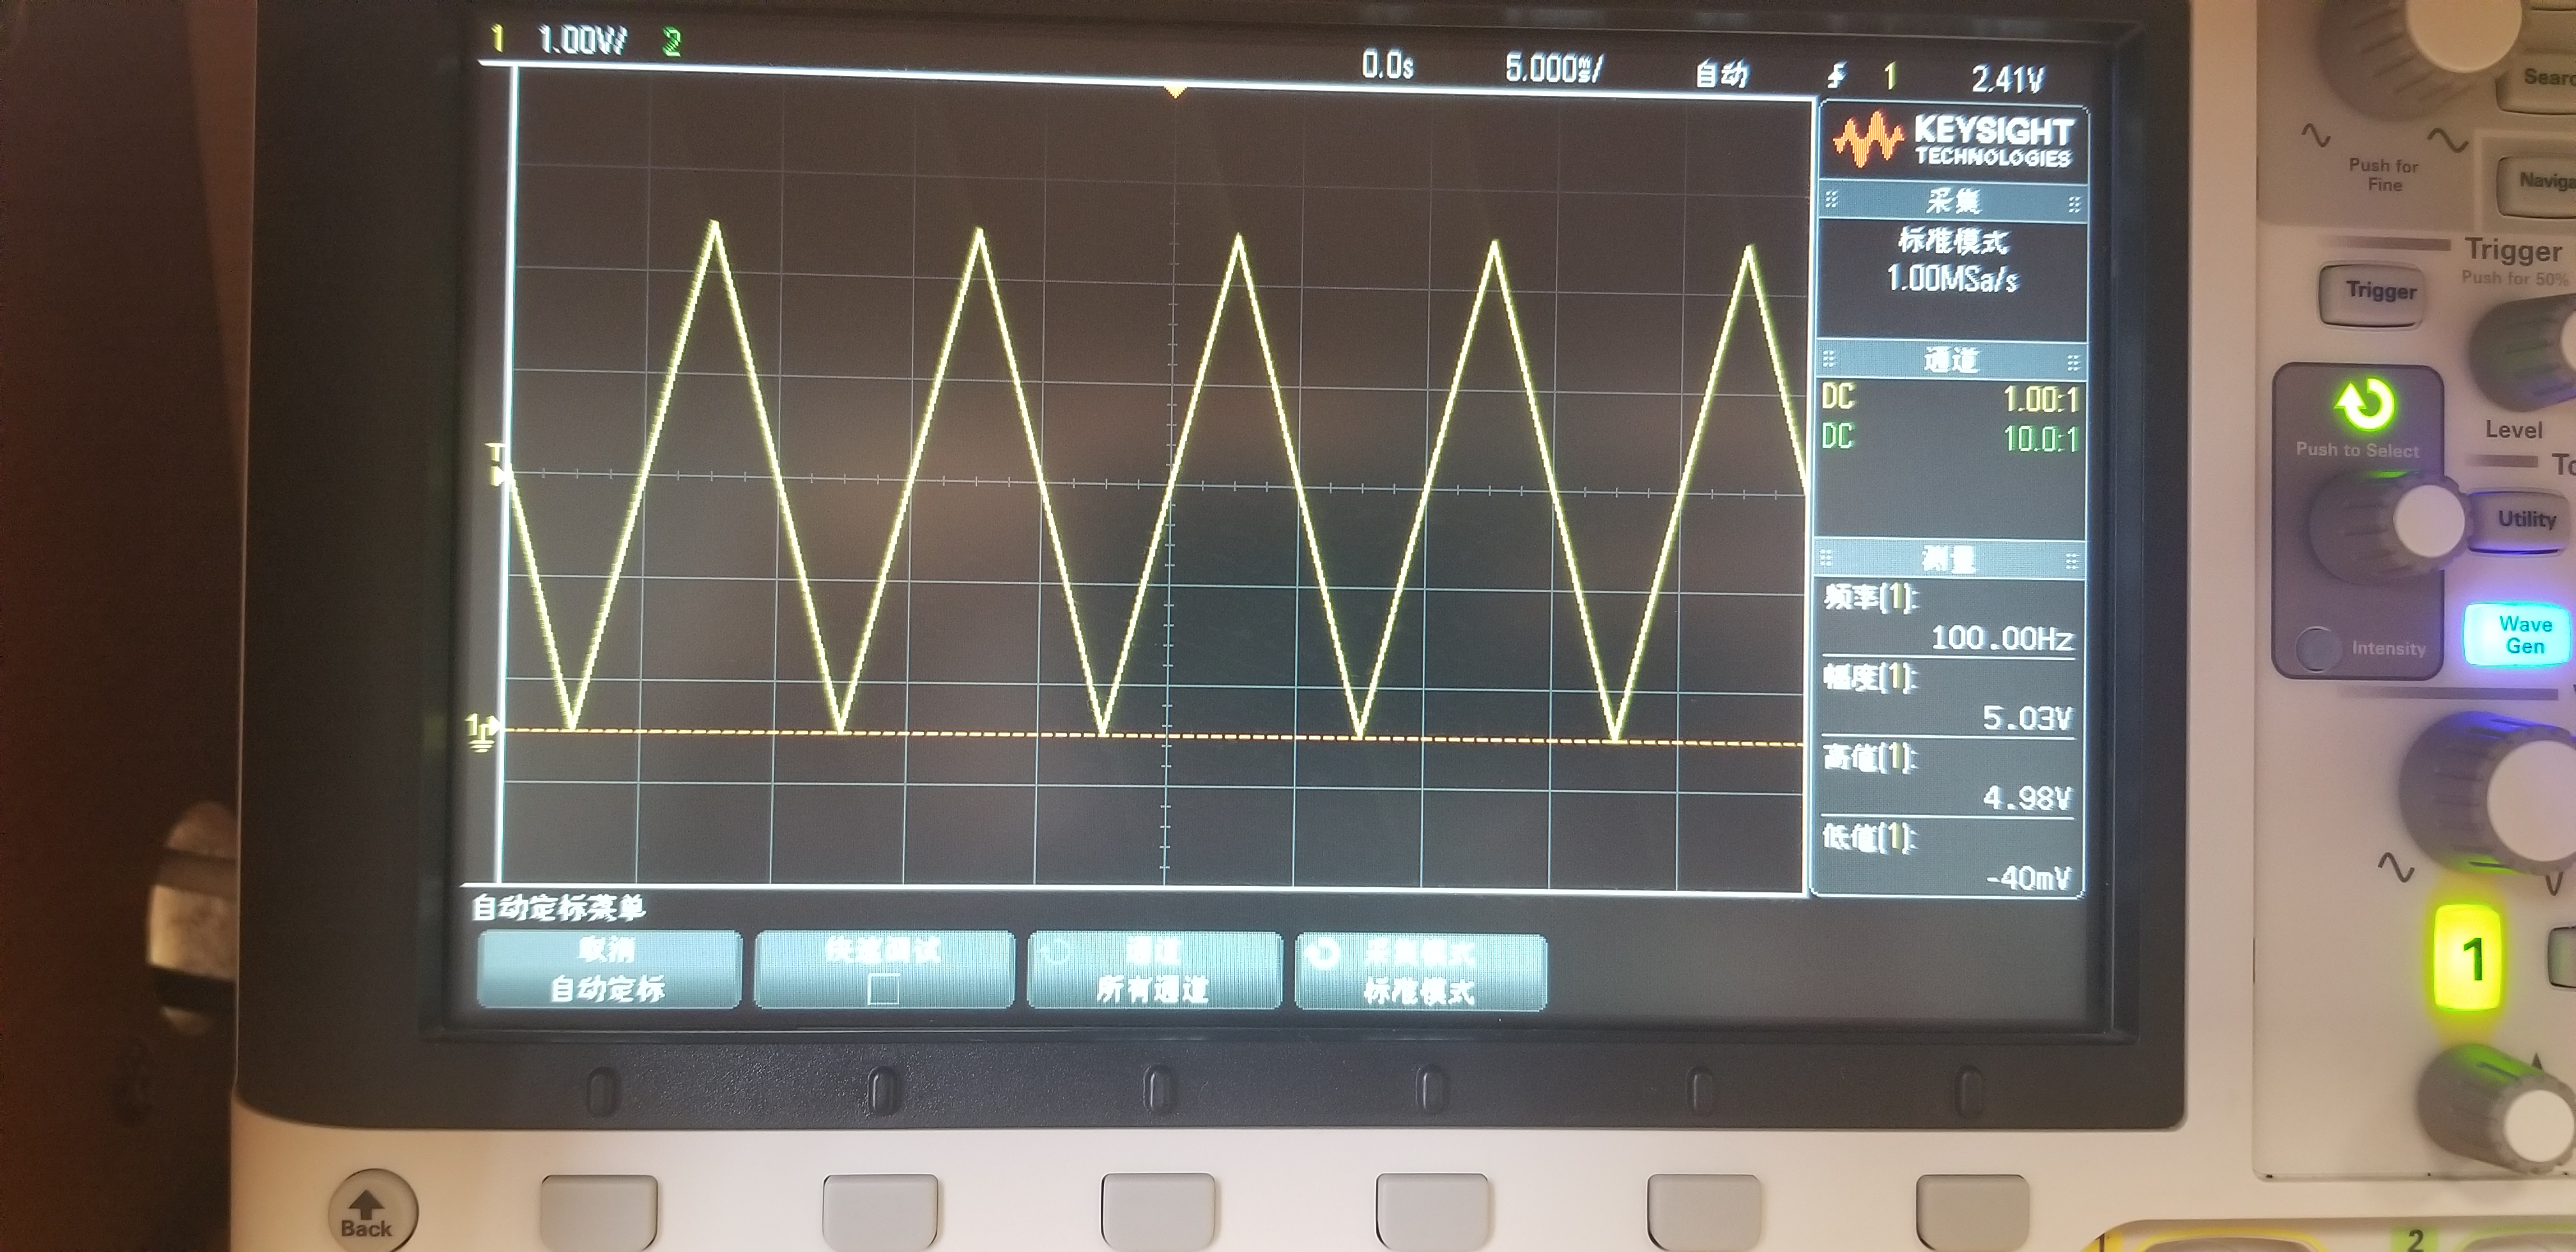
\includegraphics[width=0.7\linewidth]{figures/f3}
		\caption{三角波}
	\end{figure}

\end{document}